% Detailed, code-grounded class-specific GNN architecture.
\begingroup
\definecolor{figFiveFaceOne}{HTML}{86A9BC}
\definecolor{figFiveFaceTwo}{HTML}{F2D58A}
\definecolor{figFiveFaceThree}{HTML}{F0B078}
\definecolor{figFiveFaceFour}{HTML}{E9A4A0}
\definecolor{figFiveRivet}{HTML}{648BA4}
\definecolor{figFiveSurface}{HTML}{BD8155}
\definecolor{figFiveInk}{HTML}{354553}
\definecolor{figFiveNeutral}{HTML}{F3F5F7}
\begin{tikzpicture}[x=1mm,y=1mm,
  font=\sffamily\fontsize{7.6}{9}\selectfont,
  text=figFiveInk,
  panel/.style={font=\sffamily\fontsize{9}{10.5}\selectfont,anchor=west},
  note/.style={font=\sffamily\fontsize{7}{8.5}\selectfont,align=center},
  flow/.style={-{Latex[length=1.7mm,width=1.15mm]},draw=figFiveInk!75,
    line width=.55pt,line cap=round,line join=round},
  module/.style={draw=figFiveInk!40,fill=white,rounded corners=1.5mm,line width=.5pt,
    minimum height=19mm,inner sep=1mm,align=center},
  op/.style={draw=figFiveInk!45,fill=white,rounded corners=1mm,line width=.5pt,
    minimum height=7mm,inner sep=.7mm,align=center,
    font=\sffamily\fontsize{7}{8}\selectfont}]
  \path[use as bounding box] (0,4) rectangle (160,-177);
  \foreach \cy in {1,-49,-127} {
    \draw[draw=figFiveRivet,line width=1.6pt,line cap=round]
      (0,\cy-1.3) -- (0,\cy+1.3);
  }
  \draw[draw=figFiveSurface,line width=1.6pt,line cap=round]
    (107,-128.3) -- (107,-125.7);
  \node[panel] at (2,1) {(a) B-Rep and shared graph input};
  \node[inner sep=0] at (29,-20)
    {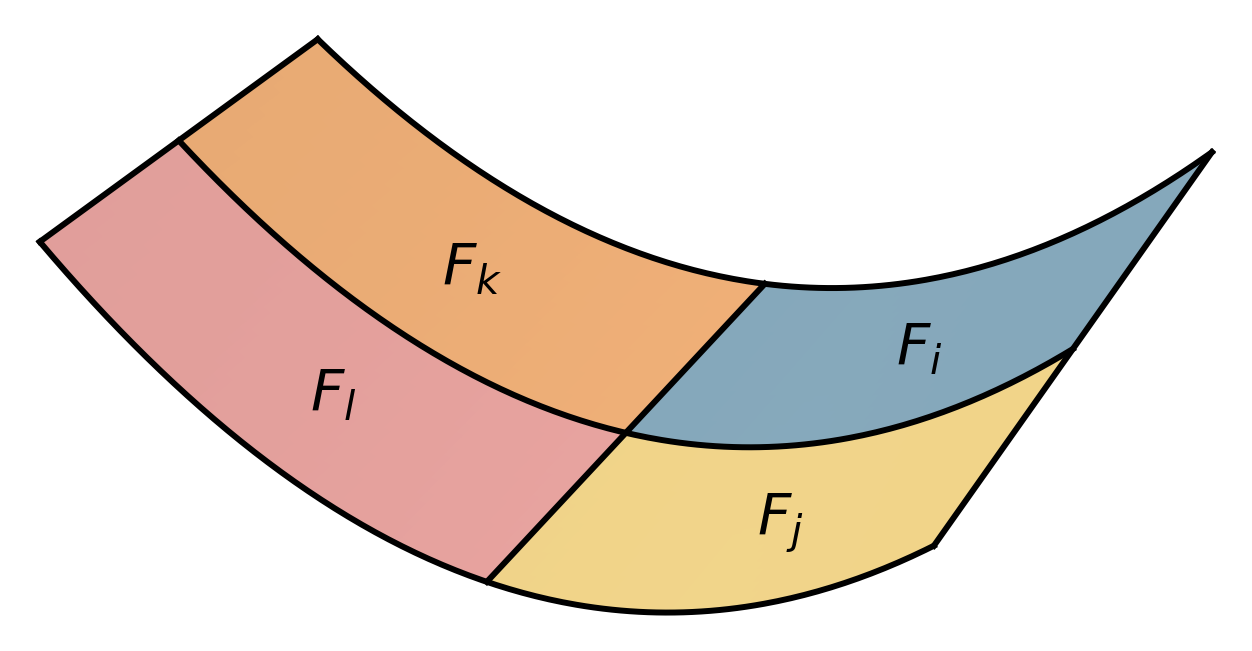
\includegraphics[width=49mm]{figures/fig5_bspline_curved_sheet.png}};
  \node[note] at (29,-38) {Four original B-Rep faces};
  \draw[flow] (56,-20) -- (66,-20);
  \draw[figFiveInk!65,line width=.6pt] (71,-15) -- (87,-15) -- (87,-27) -- (71,-27) -- cycle;
  \foreach \x/\y/\c/\f in {71/-15/figFiveFaceThree/F3,87/-15/figFiveFaceOne/F1,71/-27/figFiveFaceFour/F4,87/-27/figFiveFaceTwo/F2} {
    \node[circle,draw=figFiveInk!70,fill=\c,line width=.55pt,
      minimum size=6mm,inner sep=0] at (\x,\y) {\f};
  }
  \node[note] at (79,-38) {Face-adjacency graph};
  \draw[flow] (92,-20) -- (111,-20);
  \node[module,minimum width=43mm,minimum height=23mm,fill=figFiveNeutral] (input) at (135,-20)
    {Node attributes: $\mathbf{x}_i\in\mathbb{R}^{48}$\\[1mm]
     Edge attributes: $\mathbf{e}_{ij}\in\mathbb{R}^{6}$\\[1mm]
     Shared graph connectivity};
  \draw[flow] (input.south) -- (135,-43) -- (0,-43) -- (0,-104) -- (7,-104);
  \draw[flow] (0,-70) -- (7,-70);
  \node[note,fill=white,inner sep=.5mm] at (76,-43) {Same inputs; independently learned parameters};
  \node[panel] at (2,-49) {(b) Two class-specific branches};

  % Each branch owns all encoders, message-passing layers, adapter and head.
  \foreach \cy/\col/\branch/\k/\score in {-70/figFiveRivet/Rivet branch/r/{p_{r,i}},-104/figFiveSurface/Surface-feature branch/s/{p_{s,i}}} {
    \draw[draw=\col,fill=\col!4,rounded corners=2mm,line width=.7pt]
      (4,\cy+16) rectangle (136,\cy-13);
    \begin{scope}
      \clip[rounded corners=2mm] (4,\cy+16) rectangle (136,\cy-13);
      \fill[\col!13] (4,\cy+16) rectangle (136,\cy+9.8);
    \end{scope}
    \node[anchor=west,text=\col!65!black,font=\sffamily\fontsize{8.5}{10}\selectfont]
      at (7,\cy+12) {\branch};
    \node[module,draw=\col!80,minimum width=28mm] (enc\k) at (21,\cy)
      {Node encoder\\$\phi_{x,\k}(\mathbf{x}_i)$\\[.7mm]
       Edge encoder\\$\phi_{e,\k}(\mathbf{e}_{ij})$};
    \node[module,draw=\col!80,fill=\col!7,minimum width=30mm] (mp\k) at (57,\cy)
      {Graph encoding\\[.8mm]$4\times$ NNConv\\[.8mm]Hidden width: 64};
    \node[module,draw=\col!80,minimum width=28mm] (pool\k) at (92,\cy)
      {Mean + Max\\graph pooling\\[.7mm]Concat local/global\\$64+128\rightarrow192$};
    \node[module,draw=\col!80,minimum width=23mm] (head\k) at (122,\cy)
      {Adapter\\$192\rightarrow96$\\[.7mm]Linear $96\rightarrow1$\\Sigmoid $\sigma$};
    \draw[flow] (enc\k.east) -- (mp\k.west);
    \draw[flow] (mp\k.east) -- (pool\k.west);
    \draw[flow] (pool\k.east) -- (head\k.west);
    \node[draw=\col,fill=\col!18,line width=.6pt,rounded corners=1.5mm,
      minimum width=13mm,minimum height=11mm,inner sep=.5mm] (score\k) at (146,\cy) {$\score$};
    \draw[flow] (head\k.east) -- (score\k.west);
  }

  \node[panel] at (2,-127) {(c) Graph-convolution unit};
  \draw[draw=figFiveInk!35,fill=figFiveNeutral,rounded corners=2mm,line width=.5pt]
    (4,-132) rectangle (102,-169);
  \node[note,anchor=west] at (7,-138) {$\tilde{\mathbf{e}}_{ij,k}$};
  \node[op,fill=figFiveRivet!8,minimum width=19mm] (edgeweights) at (29,-138) {Edge MLP};
  \draw[flow] (17,-138) -- (edgeweights.west);
  \node[note,anchor=west] at (42,-138) {Edge-conditioned weights};
  \node[op,fill=figFiveRivet!8,minimum width=18mm] (conv) at (29,-153) {NNConv};
  \node[op,minimum width=9mm] (norm) at (48,-153) {LN};
  \node[op,minimum width=12mm] (relu) at (63,-153) {ReLU};
  \node[op,minimum width=16mm] (drop) at (81,-153) {Dropout};
  \node[circle,draw=figFiveInk!65,fill=white,line width=.5pt,
    minimum size=4mm,inner sep=0] (add) at (96,-153) {$+$};
  \node[note] at (12,-148) {$\mathbf{h}^{(\ell)}_{i,k}$};
  \draw[flow] (7,-153) -- (conv.west);
  \draw[flow] (edgeweights.south) -- (conv.north);
  \draw[flow] (conv.east) -- (norm.west);
  \draw[flow] (norm.east) -- (relu.west);
  \draw[flow] (relu.east) -- (drop.west);
  \draw[flow] (drop.east) -- (add.west);
  \draw[flow] (add.east) -- (101,-153);
  \draw[flow,draw=figFiveRivet] (7,-153) -- (7,-164) -- (96,-164) -- (add.south);
  \node[note,fill=figFiveNeutral,inner sep=.5mm] at (50,-164) {Residual skip: layers 2--4};
  \node[note] at (53,-174) {LN: LayerNorm. The first layer maps $48\rightarrow64$ without a skip.};

  \node[panel] at (109,-127) {(d) Score fusion};
  \node[draw=figFiveInk!45,fill=figFiveNeutral,line width=.6pt,rounded corners=2mm,
    minimum width=47mm,minimum height=14mm,align=center] (fusion) at (133,-141)
    {Rivet precedence\\$\tau_r=0.9,\quad\tau_s=0.5$};
  \draw[flow,draw=figFiveRivet] (scorer.east) -- (158,-70) -- (158,-141) -- (fusion.east);
  \draw[flow,draw=figFiveSurface] (scores.south) -- (146,-130) -- (145,-130) -- (145,-134);
  \draw[flow] (fusion.south) -- (133,-150);
  \draw[draw=figFiveInk!30,fill=figFiveNeutral!50,rounded corners=1.5mm,line width=.5pt]
    (109,-150) rectangle (157,-174);
  \foreach \cy/\col/\label in {-154/gray/Background,-162/figFiveRivet/Rivet,-170/figFiveSurface/Surface-feature} {
    \node[draw=\col!80,fill=\col!12,rounded corners=1mm,line width=.5pt,
      minimum width=41mm,minimum height=6mm,inner sep=.5mm] at (133,\cy) {\label};
  }
  \node[note] at (133,-179) {Three-class output};
\end{tikzpicture}
\endgroup
